\section{Results}
\subsection{Quantile regression estimates for panel and local models}
To analyze the relationship between systemic risks, macroprudential policy, and GDP growth, we use the model estimates of \autoref{eq:panel_qr} and \autoref{eq:local_qr} as the foundation for the comparisons. \autoref{fig:arm_qr_f_r2} and \autoref{fig:panel_r2} illustrate the goodness of fit of the local and panel quantile regression models respectively across various quantiles and horizons. Specifically, horizons 4, 8, and 12 represent GDP growth projections for 1, 2, and 3 years ahead. The models demonstrate optimal in-sample performance at the lower and upper quantiles of the GDP growth distribution. This outcome is by design since our focus is on tail risks. In the panel model, the strongest fit occurs when predicting GDP growth 2-3 years ahead, whereas the local model excels in forecasting 1-2 years ahead. This may suggest that the lag between systemic risk buildup and its materialization is shorter in Armenia compared to other countries. Therefore, we adopt the 1-year ahead estimates as the primary benchmark for our comparisons and discussions.
\begin{figure*}
    \centering 
    
\includegraphics[width=1\textwidth, angle=0]{Figures/arm_qr_f_r2.png}   
    \caption{Pseudo r-squared for local quantile regression estimates across quantiles and horizons. OLS r-squared is displayed as a dashed line. Note: generally, quantile regression and OLS (pseudo) r-squared are not comparable. They are here for convenience.}
    \label{fig:arm_qr_f_r2}%
\end{figure*}
\begin{figure*}
    \centering 
    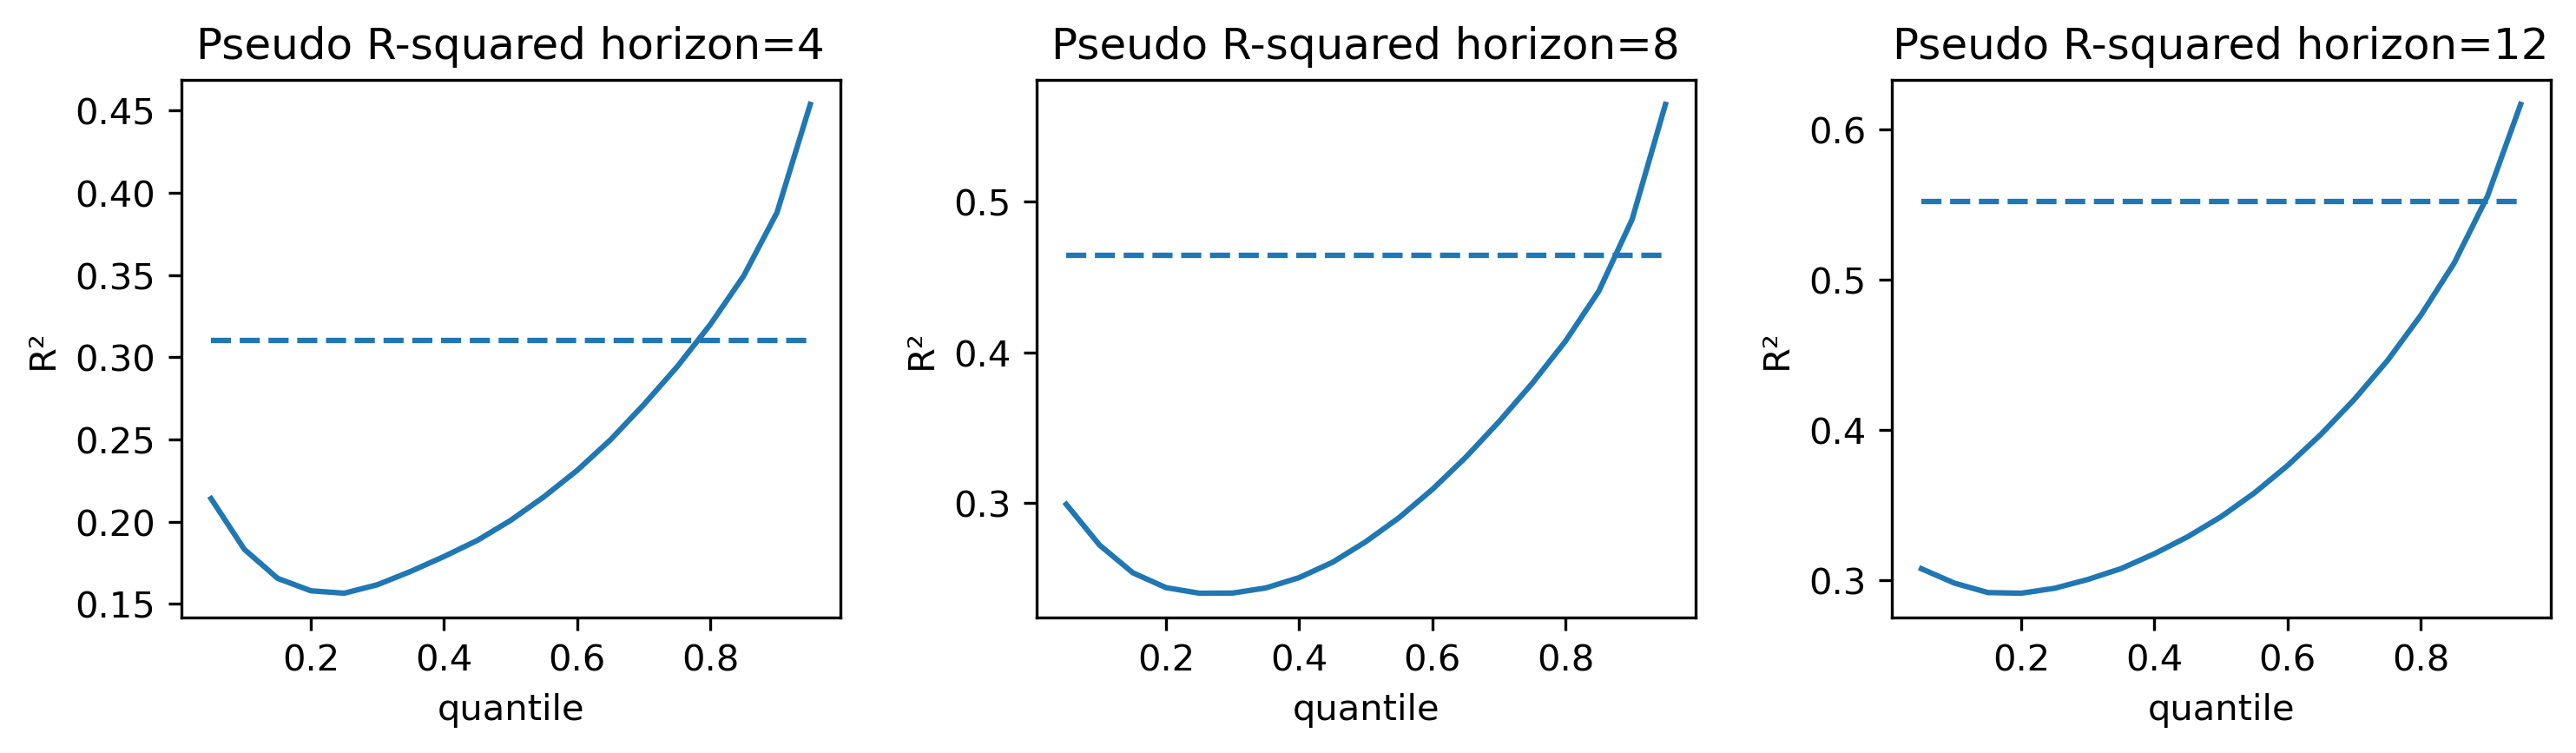
\includegraphics[width=1\textwidth, angle=0]{Figures/panel_r2.png}  
    \caption{Pseudo r-squared for panel quantile regression estimates across quantiles and horizons. OLS r-squared is displayed as a dashed line.} 
    \label{fig:panel_r2}%
\end{figure*}
\begin{figure*}
    \centering
    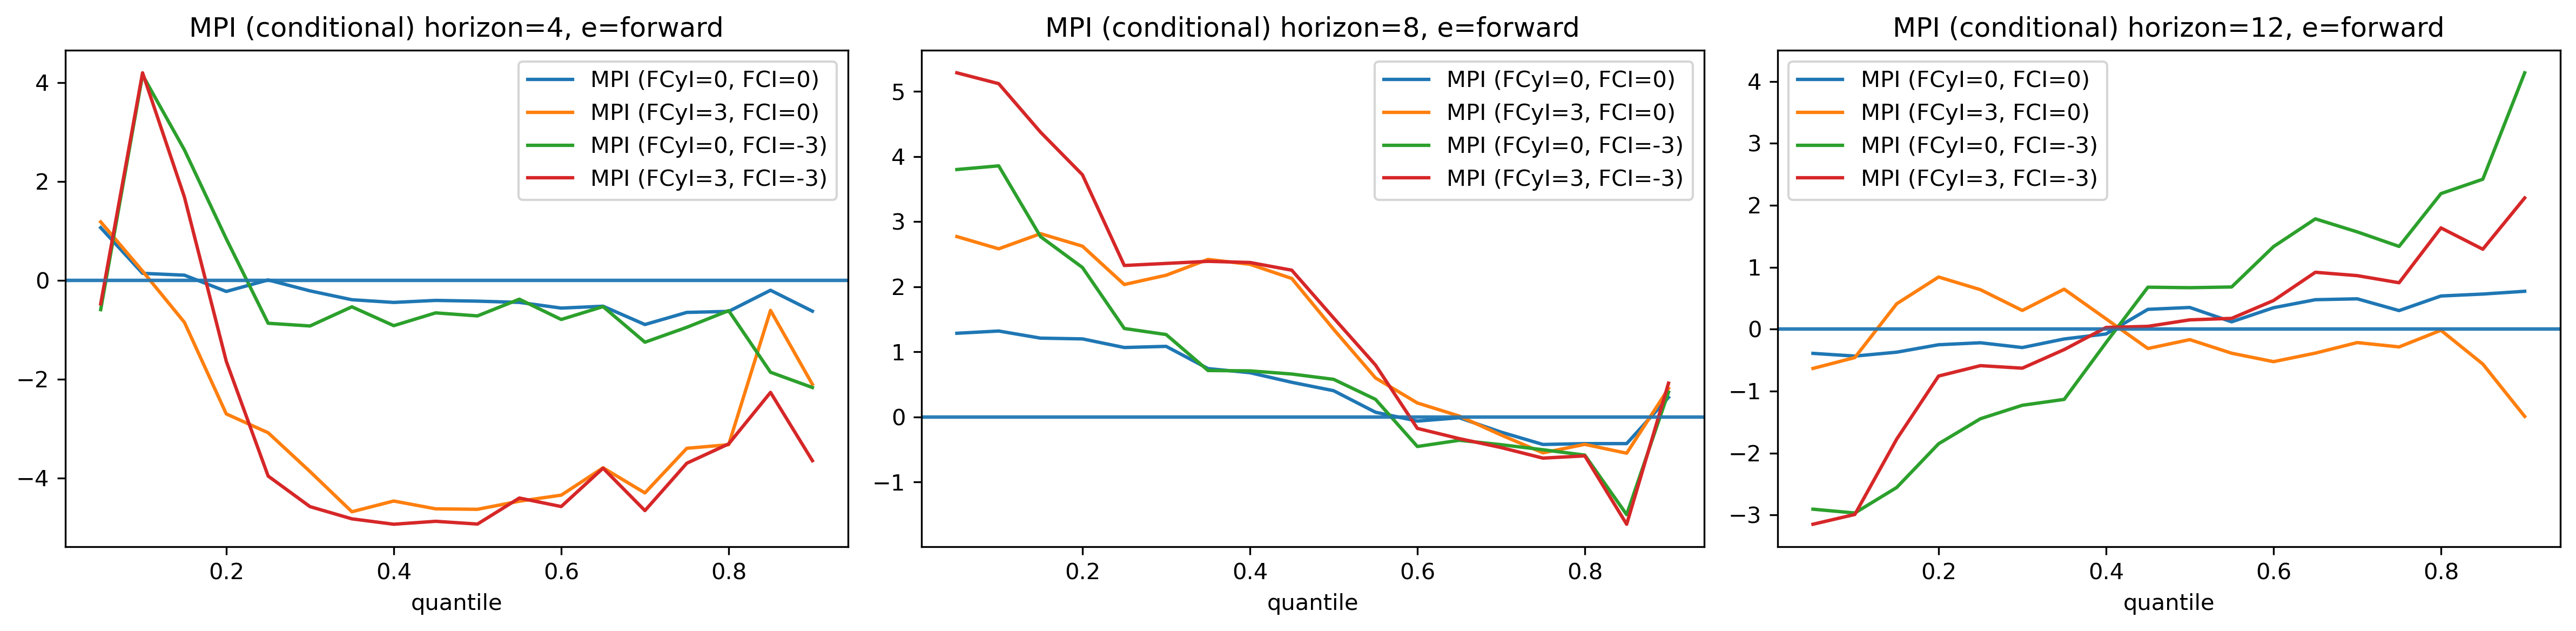
\includegraphics[width=1\textwidth, angle=0]{Figures/arm_MPI_cond_coeff_quantiles.png}  
    \caption{Local model conditional Macroprudential Policy Index coefficients. Estimated quantile regression coefficients for horizons 4, 8 and 12.}
    \label{fig:arm_MPI_cond_coeff_quantiles}%
\end{figure*}

\autoref{fig:arm_FCyI_f_coeff_quantiles} and \autoref{fig:panel_FCyI_coeff_quantiles} display the quantile regression coefficients for the FCyI in the local and panel models, respectively. In the local model, the FCyI shows a negative but insignificant effect in the short run, while its negative impact becomes significant over the long run. Conversely, the panel model demonstrates a consistently negative and significant FCyI effect in both the short and long run.

Additionally, the results reveal heterogeneous effects of FCyI across the distribution, with more pronounced impacts in the lower quantiles. This indicates that increases in FCyI exacerbate tail risks, suggesting that it would increase distance-to-tail, which is in line with the theory of business and financial cycles where a maturity or a peak phase is followed by a contraction. The results suggest that financial vulnerabilities affect the economy in the medium term. This relationship was also observed in Portugal where credit aggregates were the most relevant medium term predictors of future GDP growth \citep{imf_gar_2019}.

\autoref{fig:arm_FCI_f_coeff_quantiles} and \autoref{fig:panel_FCI_coeff_quantiles} present the quantile regression coefficients for the FCI in both the local and panel models. In the local model, the FCI is positive and largely significant in the short run but becomes insignificant over the long-term. In contrast, the panel model shows that FCI remains significant across both time dimensions, though its effect varies considerably. The FCI negatively impacts the left and right tails while positively influencing the middle quantiles.

A high FCI reflects tight financial conditions. In the near term, this effect should be negative, yet due to its cyclical and mean-reverting nature, it will eventually normalize, boosting future growth \citep{imf_gar_2019}. The positive short-term coefficient in the local model likely reflects this cycle, where financial stress is followed by economic recovery. Meanwhile, the negative effect on the left tail in the panel model underscores the long-term negative externalities that financial stress can create. Overall, the literature suggests that FCI should primarily exert short-term effects on the GDP growth distribution \citep{esrb2021}.

\subsection{The impact of macroprudential policy on output growth distribution}
Macroprudential policy enters the panel and local equations through both direct and indirect (interaction) effects. Direct effects capture the benefits of increased resilience from policy interventions, as well as the associated costs. Interaction effects, on the other hand, capture the role of macroprudential policy in mitigating systemic risks in various situations and times (e.g. when cycle is up or down, or when stress level is elevated or low).

\autoref{fig:arm_MPI_f_coeff_quantiles} and \autoref{fig:panel_MPI_coeff_quantiles} plot the quantile regression coefficients for the direct effects of MPI in the local and panel models, respectively. In the local model, the short-run direct effects are positive at the left tail and negative at the median, though these coefficients are statistically insignificant. The panel model shows similar short-run patterns but with significant effects. Lastly, the long-run direct effects are negative and significant. 

The heterogeneity in the direct effects suggests that, in the short run, MPI improves resilience and reduces distance-to-tail. However, if financial conditions remain stable and no crisis is observed, MPI could have negative long-term implications for both the median and distance-to-tail. These outcomes reflect the practical costs of macroprudential policy \citep{schmitz2022eu}, but also the prolonged requirement for banks to hold excess capital, which may suppress economic activity over time.

To examine the overall impact of macroprudential policy, we present the conditional MPI coefficients in \autoref{fig:arm_MPI_cond_coeff_quantiles}. The reason behind this definition is the convention, that the effectiveness and magnitude of performed policy actions will be heavily dependent on the conditions present in the system: whether it is early stage of financial cycle and risks are largely in neutral level or below it, or the system is operating at the peak of financial cycle, where significant amount of risks are accumulated. The situation is further complemented by the level of stress in the system. This has been done by defining a special function, which takes the baseline estimation from the model and transforms it according to the priors we provide for both FCyI and FCI (basically these priors are presented in the figure with numbers: -3 stands for underperformance, 0 for neutral level and 3 for overheating or elevated level of risks).

Short-term effects highlight the negative inpact that macroprudential policy can have on median GDP growth, which is essentially the short-term cost of macroprudential on future GDP growth. On the other hand, the long-term results suggest, that in the longer term, the tail of GDP distribution shrinks significantly, while significantly benefitting the right tail of distribution. The rightmost chart in \autoref{fig:arm_MPI_cond_coeff_quantiles} also suggests that macroprudential policy is most effective during periods of low financial stress (red and green lines in the chart). However, if such periods coincide with excessive credit growth or asset price surges, the short-term costs to growth will be higher (coefficient value for median on red line in leftmost chart). Nonetheless, these conditions also lead to the most significant reduction of risks in the medium term.
